Node.js es un entorno multiplataforma de código abierto para ejecutar código JavaScript del lado del servidor. El entorno de tiempo de ejecución de Node.js incluye todo lo que necesita para ejecutar un programa escrito en JavaScript. 
\vspace{0.8cm}

Node.js surgió cuando los desarrolladores originales de JavaScript lo extendieron de algo que solo podía ejecutar en el navegador a algo que podría ejecutar en su máquina como una aplicación independiente. Ahora puede hacer mucho más con JavaScript que simplemente hacer que los sitios web sean interactivos. JavaScript ahora tiene la capacidad de hacer cosas que otros lenguajes de secuencias de comandos como Python pueden hacer. Tanto su navegador JavaScript como Node.js se ejecutan en el motor de tiempo de ejecución JavaScript V8. Este motor toma su código JavaScript y lo convierte en un código de máquina más rápido. El código de máquina es un código de bajo nivel que la computadora puede ejecutar sin necesidad de interpretarlo primero.
\begin{figure}[H]
  \centering
  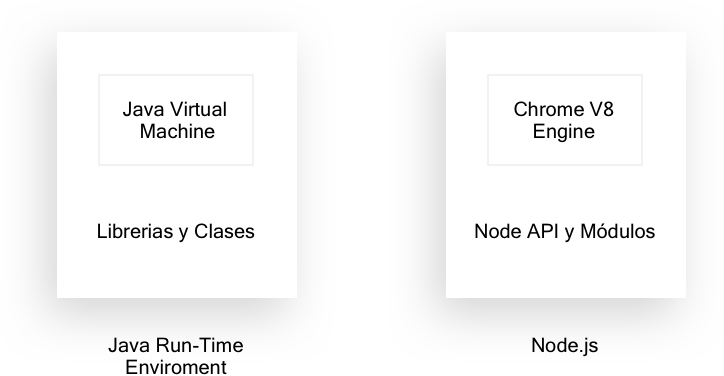
\includegraphics[width=0.8\textwidth]{node}
  \caption{Analogía Node.js con Java.}
\end{figure}
% \vspace{0.8cm}

\subsubsection{Motor V8 de Google Chrome}
Node.js utiliza el motor de ejecución ultra rápido V8 de Google Chrome. Hasta el lanzamiento de Chrome, la mayoría de los navegadores leían JavaScript de manera ineficiente: el código se leía e interpretaba poco a poco. Tomó mucho tiempo leer JavaScript y convertirlo a lenguaje máquina para que el procesador pudiera entenderlo. 
\vspace{0.8cm}

El motor V8 de Google Chrome funciona completamente diferente. Está altamente optimizado y lleva a cabo lo que llamamos compilación JIT (Just In Time). Transforma rápidamente el código JavaScript en lenguaje máquina.
